\section{Introduction}
\subsection{Nuclear Energy}
\frame
{
  \frametitle{Nuclear Energy Perspective}
	\begin{itemize}
		\item Nuclear power has historically been one of the largest contributors of low-carbon electricity globally.
		\item Nuclear power today makes a significant contribution to electricity generation, providing 10\% of global electricity supply in 2018.
		\item In advanced economies, nuclear power accounts for 18\% of generation and is the largest low-carbon source of electricity.
		\item Nuclear power can play an important role in clean energy transitions and it has significant potential to contribute to power sector decarbonisation\footnote{ IEA (2019), "Nuclear Power in a Clean Energy System", IEA, Paris.}.
		\item Nuclear power plants contribute to electricity security in multiple ways such as keeping power grids stable.
		\item Without nuclear investment, achieving a sustainable energy system will be much harder and offsetting less nuclear power with more renewables would cost more.
		\item A doubling in annual capacity additions is needed to be on track with the IEA's Sustainable Development Scenario\footnote{ IEA (2019), "Tracking Power", IEA, Paris.}.
	\end{itemize}
}

\frame{
	\frametitle{Nuclear Reactors}
	\onslide<1->{\begin{itemize}
		\item<1-> Nuclear reactors are used to carry out controlled chain reactions to produce heat through fission.
		\item<2-> Most of the reactors currently in use are 2\textsuperscript{nd} / 3\textsuperscript{rd}  generation Light Water Reactors or Pressurised Heavy Water Reactors.
	\end{itemize}}
	\onslide<2->{\begin{figure}[htbp]
		\begin{center}
			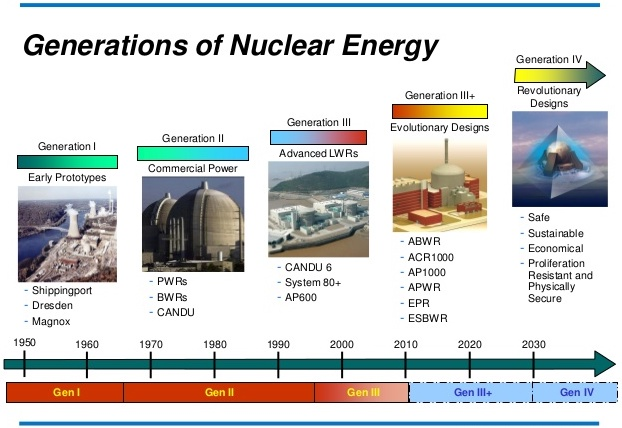
\includegraphics[height=0.5\paperheight]{Figures/Gen_Nuclear}	
		\end{center}
	\end{figure}}
}

\subsection{Generation IV Reactors}
\frame{
	\frametitle{Generation IV Reactors}
	\only<1-5>{\begin{itemize}
		\item<1-> Generation IV reactors are advanced reactor concepts under development with the following goals:
			\begin{itemize}
				\item <2-> \textbf{Sustainability}: Energy generation that meets clean air objectives and provides long-term availability of systems and effective fuel utilisation for worldwide energy production. Also, minimise and manage nuclear waste.
				\item <3-> \textbf{Economy}: A clear life-cycle cost advantage over other energy sources and a level of financial risk comparable to other energy projects.
				\item <4-> \textbf{Safety and reliability}: Excel in safety and reliability and a very low likelihood and degree of reactor core damage.
				\item <5-> \textbf{Proliferation resistance}: Increase the assurance that these systems are the least desirable route for diversion or theft of weapons-usable materials.
			\end{itemize}
	\end{itemize}}	
	\only<6>{\begin{figure}[htbp]
		\begin{center}
			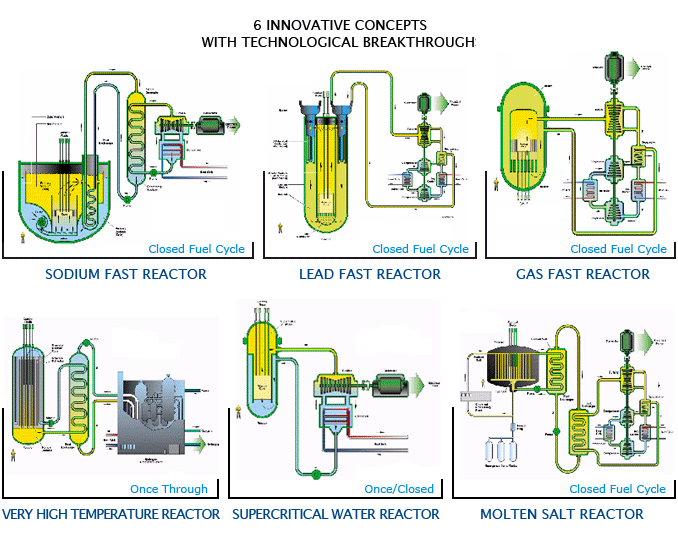
\includegraphics[width=0.75\paperwidth,height=0.65\paperheight]{Figures/gen_4_concepts}	
		\end{center}
	\end{figure}
	\blfootnote{Image - Generation IV International Forum}}
}

\frame{
	\frametitle{Molten Salt Reactor}
	\only<1-2>{\begin{itemize}
		\item Molten Salt Reactors (MSRs) are circulating fuel reactors and are one of the six concepts selected for further design and development under the Generation IV framework.
	\end{itemize}}	
	\only<2>{\begin{figure}[htbp]
		\begin{center}
			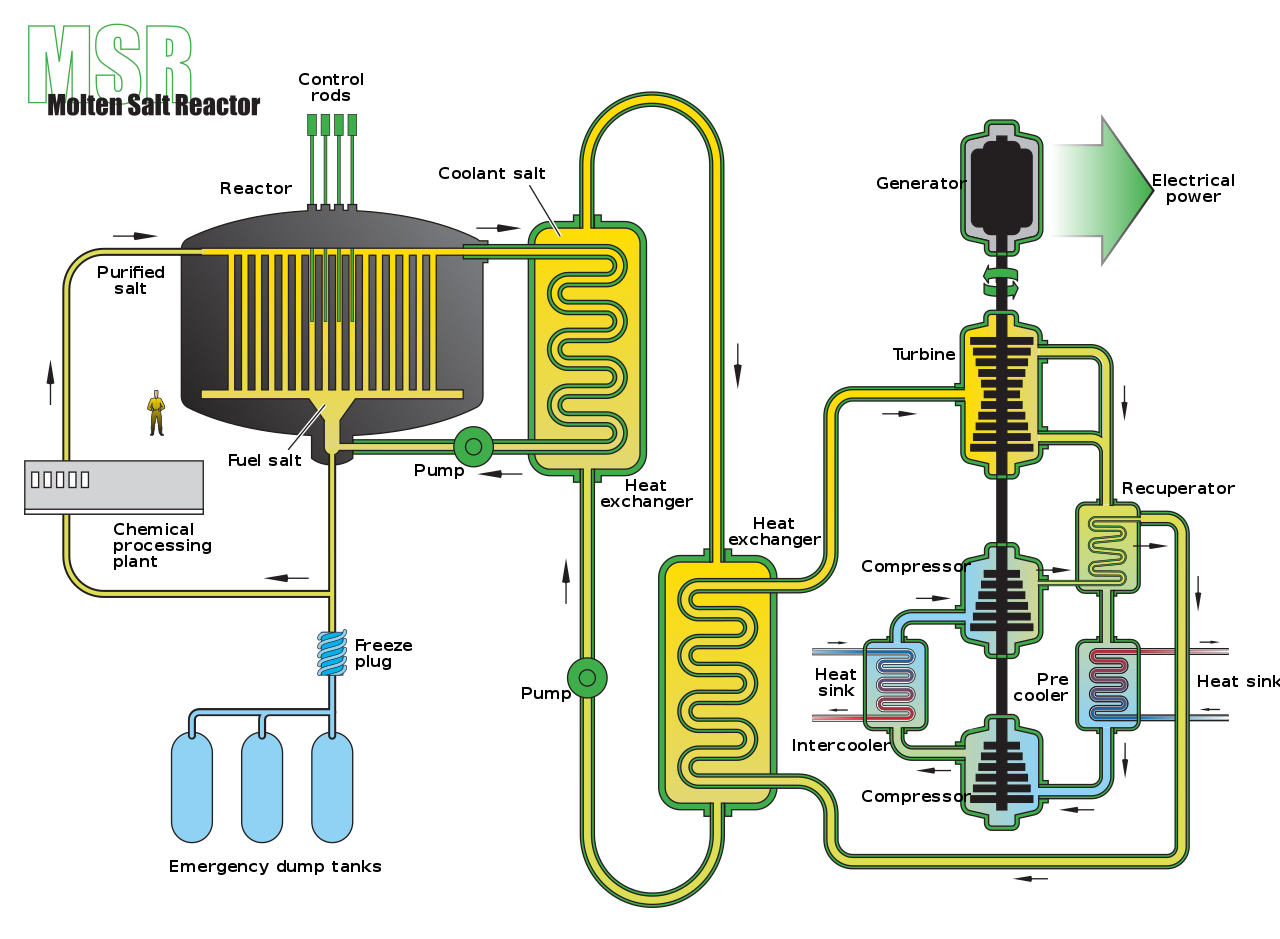
\includegraphics[height=0.55\paperheight]{Figures/MSR}	
		\end{center}
	\end{figure}
	\blfootnote{Image - Generation IV International Forum}}
	\only<3-4> 
	{\begin{itemize}
		\item MSR exhibit very tight coupling between different physical phenomena.
	\end{itemize}}	
	\only<4>{\begin{figure}[htbp]
		\begin{center}
			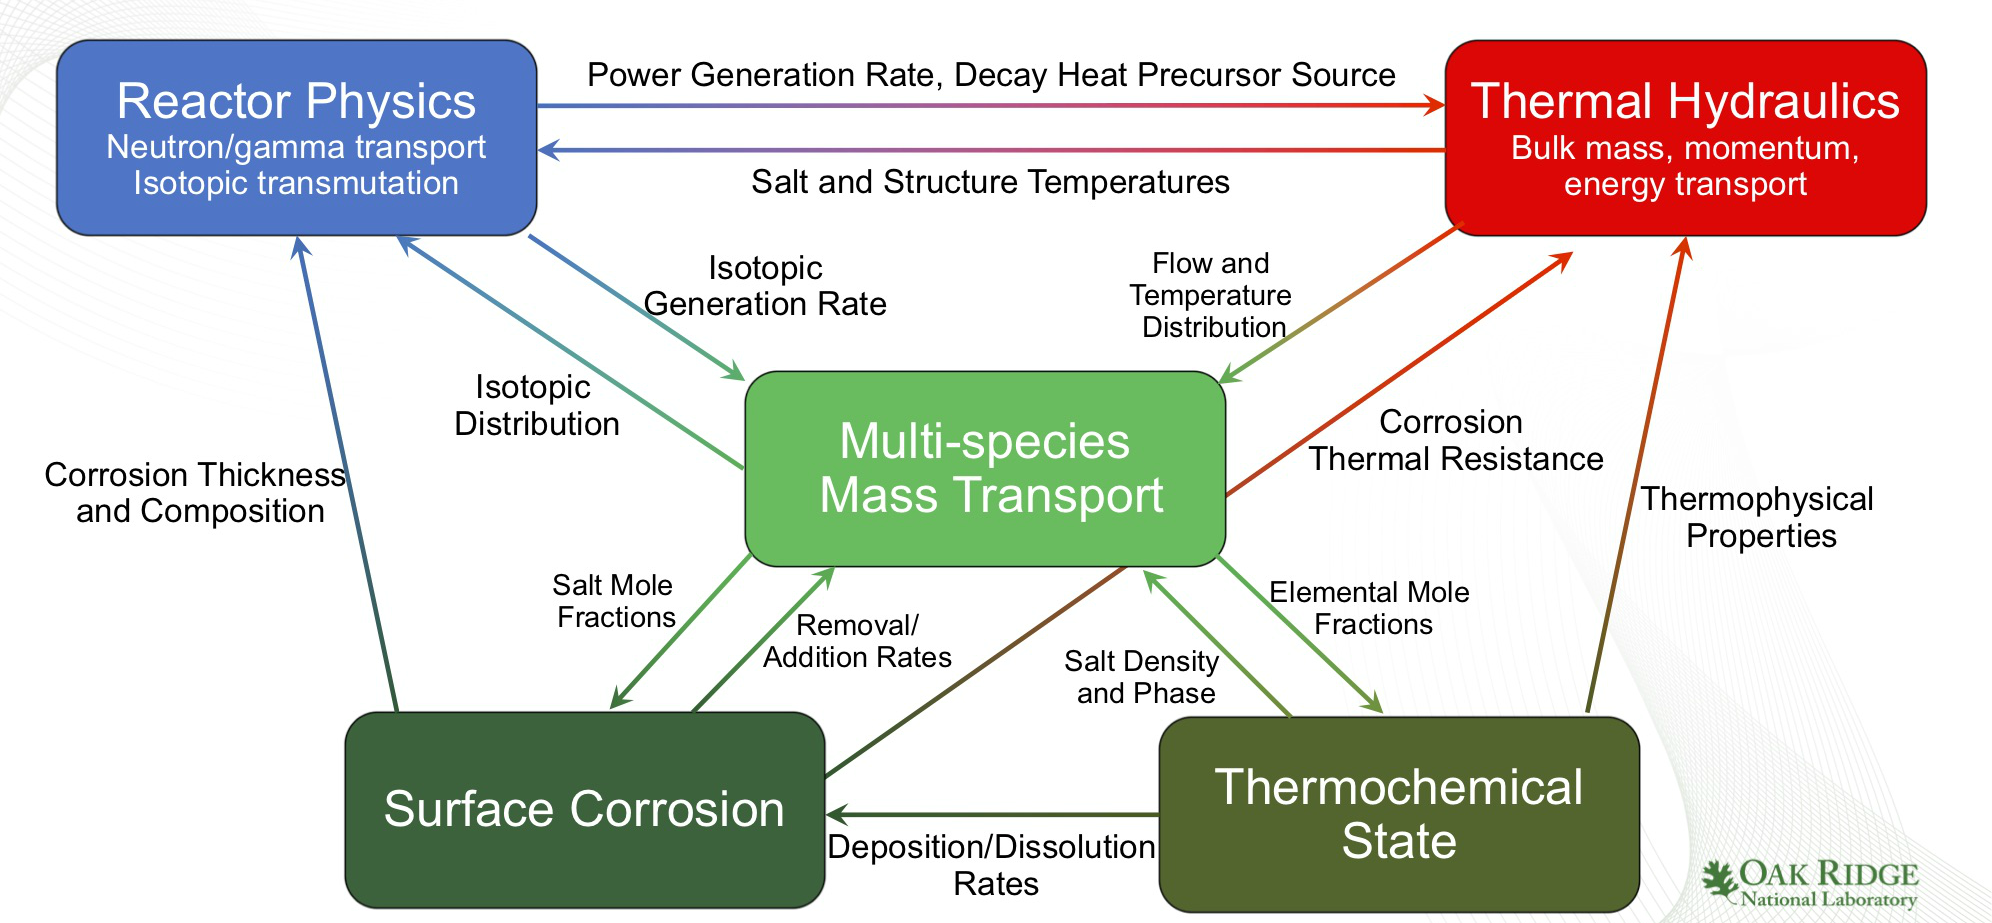
\includegraphics[height=0.55\paperheight]{Figures/MSR_MPH}	
		\end{center}
	\end{figure}
	\blfootnote{Image - B. Collins, Presentation at Oak Ridge National Laboratory.}}
}

\subsection{Multiphysics Simulations}

\frame{
	\frametitle{Simulation of Nuclear Reactors}
	\begin{itemize}
		\item Traditional reactor simulation tools rely on the \emph{Operator Splitting} approach.
	\end{itemize}
	\pause	
	\begin{figure}[htbp]
		\begin{center}
			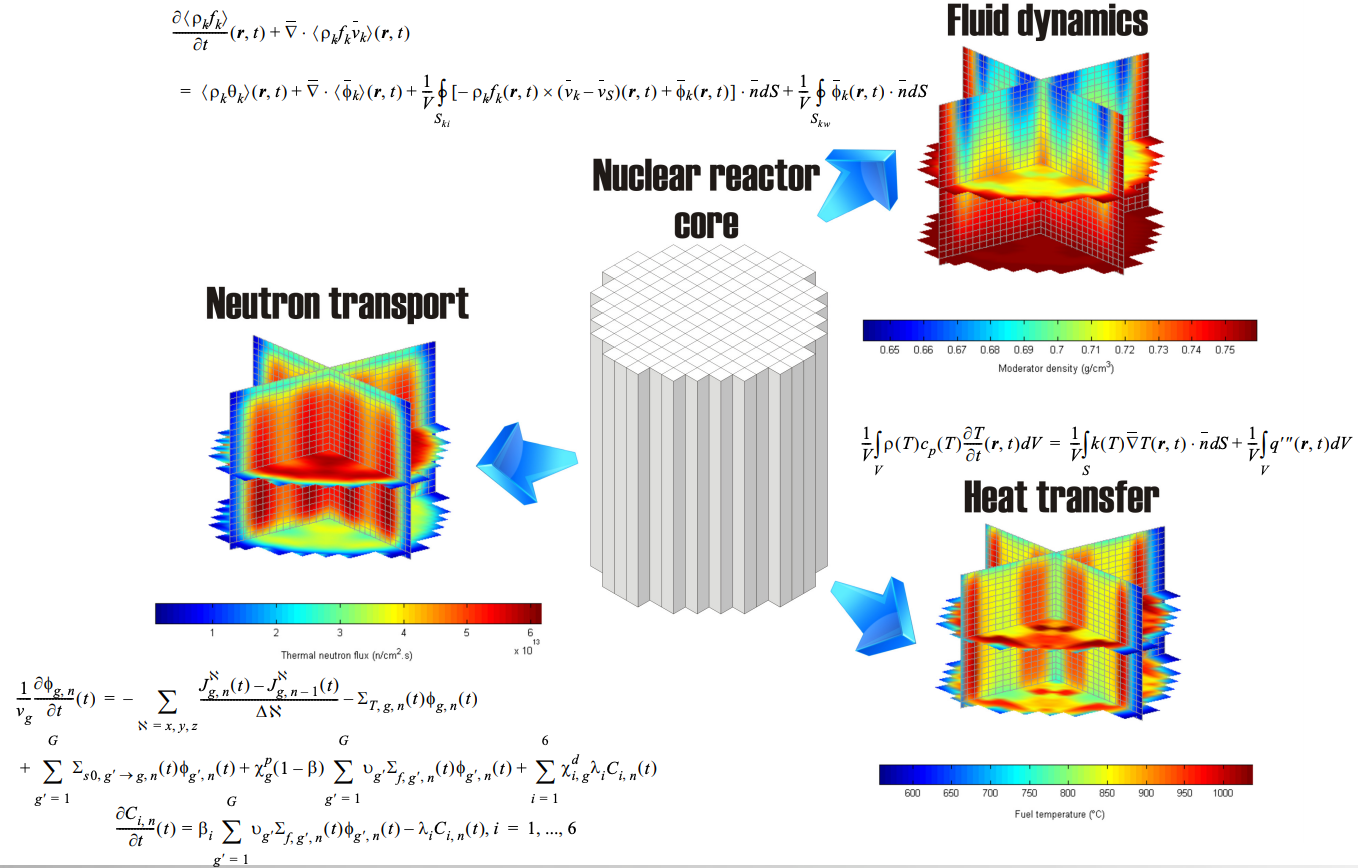
\includegraphics[height=0.55\paperheight]{Figures/Operator_split}	
		\end{center}
	\end{figure}
}

\frame{
	\frametitle{MOOSE}
	\only<1>{\begin{itemize}
		\item<1-> Design and simulation of advanced reactors requires advanced multiphysics tools.
		\item<1-> Multiphysics Object Oriented Simulation Environment (MOOSE) is a finite element framework for solving computational engineering problems.
		\item<1-> Developed for massively parallel (MPI+Threads) simulation but the user code is agnostic of parallelism.
		\item<1-> Developed by the Idaho National Laboratory and open-source since 2014.
		\item<1-> MOOSE follows a Nuclear Quality Assurance Level 1 (NQA-1) development process.
		\item<1-> MOOSE includes a test suite and documentation system to allow for agile development while maintaining a NQA-1 process.
	\end{itemize}}
	\only<2>{\begin{figure}[htbp]
		\begin{center}
			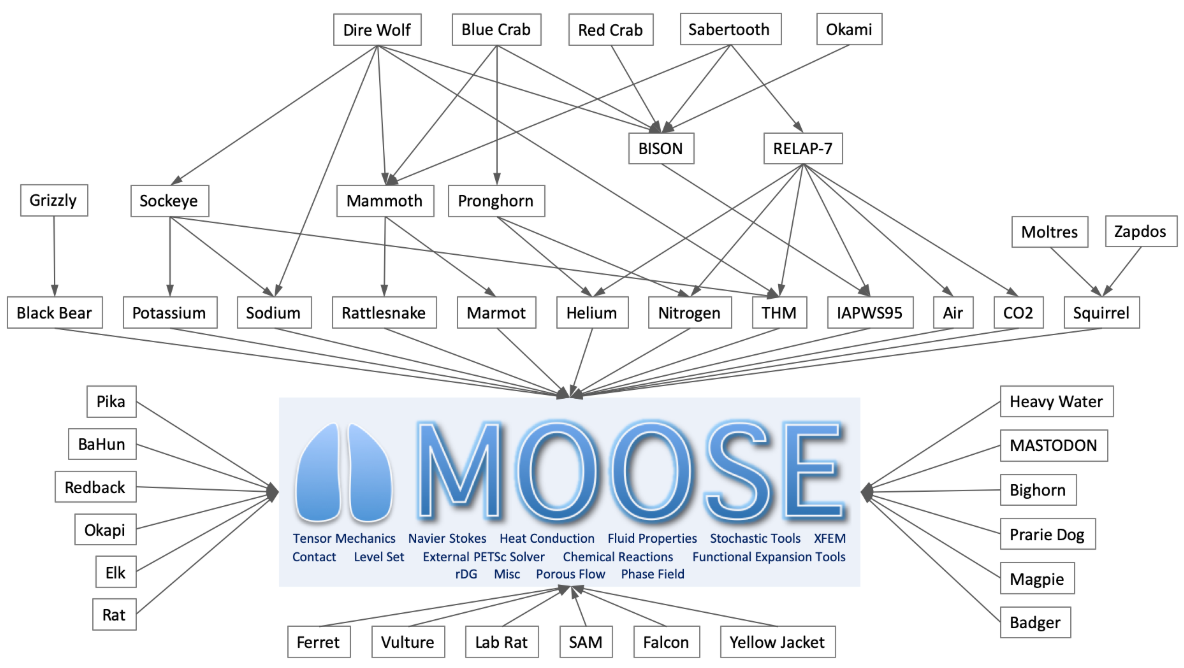
\includegraphics[width=0.85\paperwidth]{Figures/moose}	
		\end{center}
	\end{figure}
	\blfootnote{Image - MOOSE Website, \url{https://mooseframework.org/workshop/}}}
}


\frame{
	\frametitle{Nuclear Materials}
	\only<1-2>{\begin{itemize}
		\item<1-> Nuclear materials are highly complex multiscale, multiphysics systems. Design and development of nuclear materials can be supported by numerical simulations to make the process both time and cost efficient.
	\end{itemize}}
	\only<2>{\begin{figure}[htbp]
		\begin{center}
			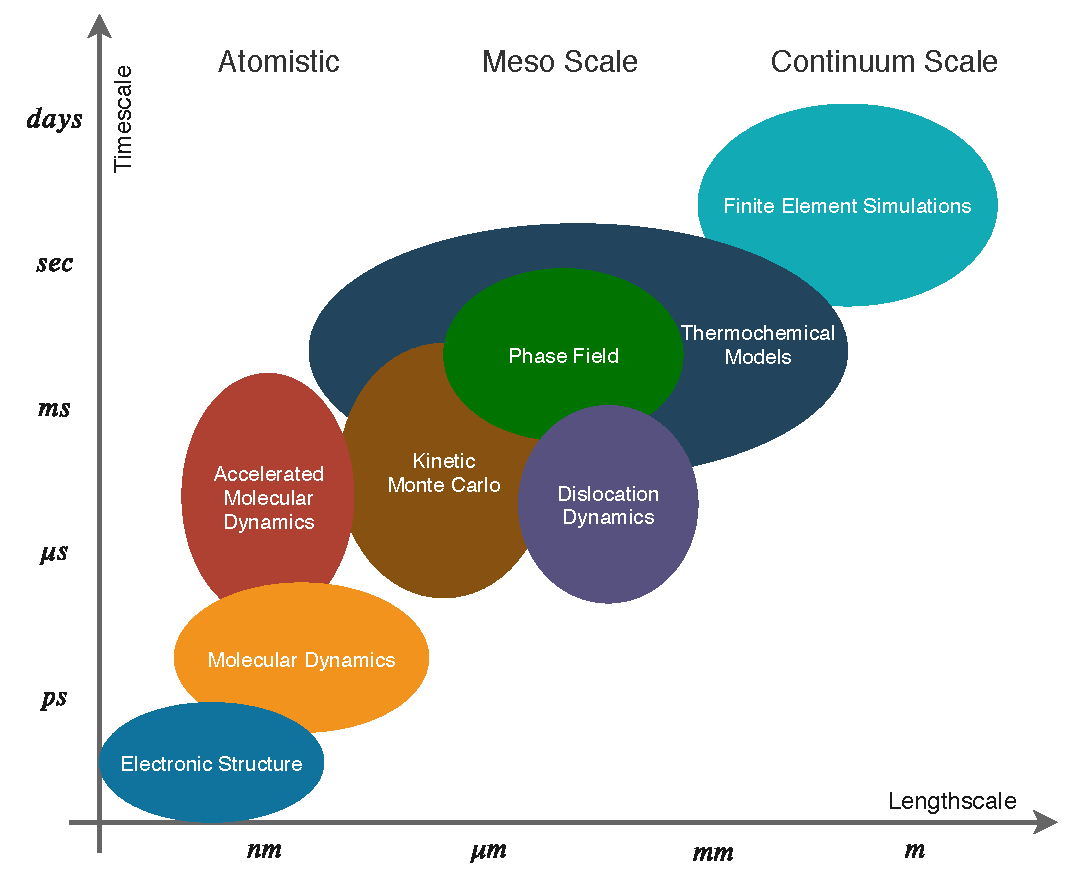
\includegraphics[height=0.5\paperheight]{Figures/Multiphysics.pdf}	
		\end{center}	
	\end{figure}
	\blfootnote{Image - M. Stan, Mater. Today, 12 (11), 20-28, 2009.}}
	\only<3>{\begin{itemize}
		\item The materials simulation tools of MOOSE form the Fuels Product Line (FPL).
		\item The framework consists of MOOSE,  fuel performance code Bison and mesoscale microstructural evolution tool Marmot.
	\end{itemize}
	\begin{figure}[htbp]
		\begin{center}
			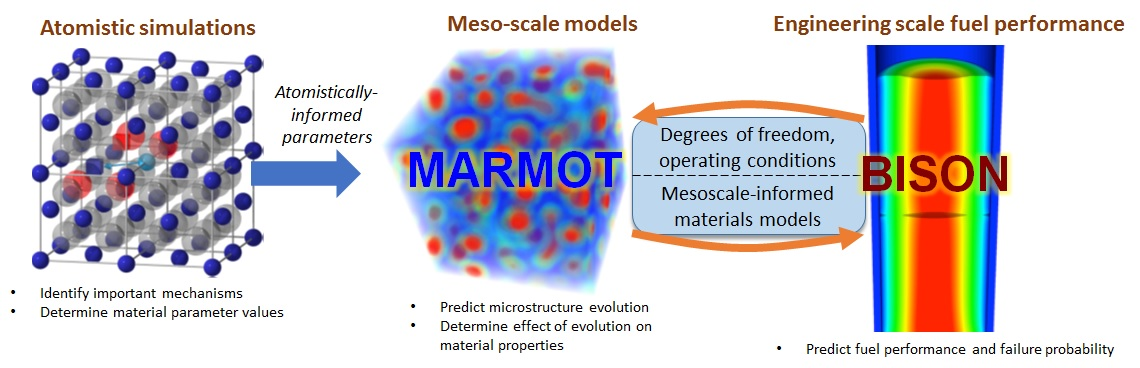
\includegraphics[width=0.85\paperwidth]{Figures/FPL}	
		\end{center}
		\end{figure}
		\blfootnote{Image - NEAMS website, \url{https://neams.inl.gov/}}}
		
}

\frame{
	\frametitle{Corrosion}
	\begin{itemize}
		\item<1-> MSRs and other advanced reactors use high temperature fluids such as molten fluoride/chloride salts.
		\item<1-> High temperature fluids especially molten fluoride/chloride salts cause corrosion of  structural materials.
		\item<1-> Corrosion is an electrochemical process driven by the thermodynamic and kinetics of the system.
		\item<1-> Effective prediction of corrosion requires a multiscale, mutiphysics approach.
	\end{itemize}
	\onslide<2->
	{\begin{alertblock}{}
		\centering {Currently, MOOSE lacks a corrosion modelling tool!}
	\end{alertblock}}
}

\frame{
	\frametitle{Yellowjacket}
	\only<1>{\begin{itemize}
		\item<1-> Yellowjacket is a new corrosion modelling tool currently under development.
		\item<1-> Yellowjacket will couple existing phase field capabilities with new thermodynamic capabilities to effectively model corrosion in advanced reactors.
		\item<1-> The primary audience for Yellowjacket is U.S. Department of Energy and molten salt reactor developers in the U.S. 
		\item<1-> Collaboration between Ontario Tech University, University of Florida, Idaho National Laboratory and Los Alamos National Laboratory.
		\item<1-> Funded by the U.S. Department of Energy through Idaho National Laboratory and the development of thermochemistry solver is also supported by the Canada Research Chairs program.
	\end{itemize}}
	\only<2->{\begin{figure}[htbp]
		\begin{center}
			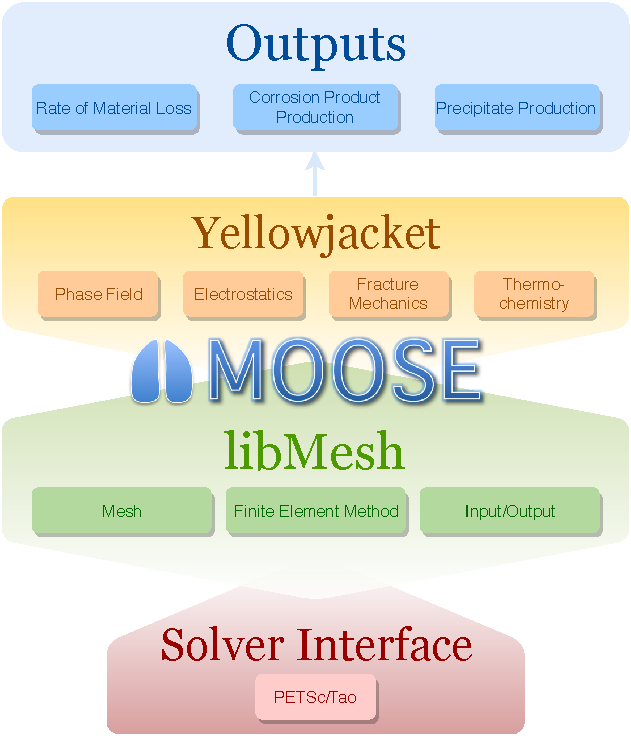
\includegraphics[height=0.7\paperheight]{Figures/Yellowjacket_MOOSE.pdf}	
		\end{center}
		\end{figure}
	}
}

\frame{
	\frametitle{Thermodynamics in Yellowjacket}
	\only<1>{\begin{itemize}
		\item<1-> Phase and chemical behaviour of nuclear materials is governed by the thermodynamic equilibrium state.
		\item<1-> The composition of nuclear materials continuously evolves under irradiation affecting the equilibrium state.
		\item<1-> Capturing thermodynamic equilibria has traditionally relied on empirical correlations.
		\item<1-> Direct coupling of thermodynamic equilibrium can augment multiphysics calculations by providing quantities such as the chemical potentials, Gibbs energies, etc. 
	\end{itemize}}
	\only<2->{\begin{figure}[htbp]
		\begin{center}
			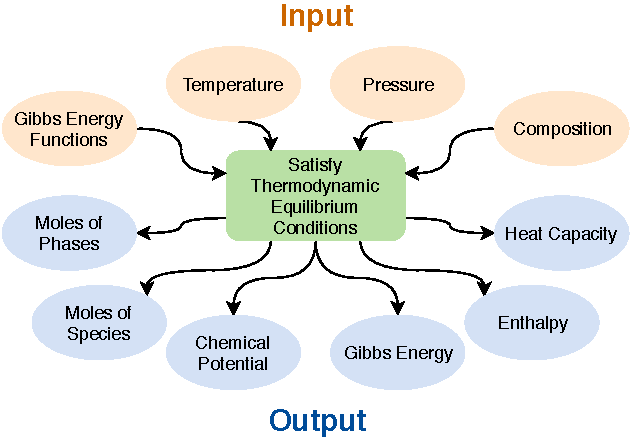
\includegraphics[height=0.75\paperheight]{Figures/Thermodynamics.pdf}	
		\end{center}
		\end{figure}
	}
}




























